\documentclass{article}
%necessary packages, use xelatex to compile
\usepackage[margin=1in]{geometry}
\usepackage{helvet}
\usepackage{xeCJK}
\usepackage{amsmath}
\usepackage{graphicx}
%changing the main font
\renewcommand{\familydefault}{\sfdefault}
%cool traditional chinese font for my name :^D
\setCJKmainfont{FandolKai-Regular.otf}

\title{Introduction to Pattern Recognition Homework 2 Report}
\author{Andr\'es Ponce(彭思安) \\
\and
0616110}
\begin{document}

\maketitle
\section{Coding}
	\subsection{Compute the mean vectors $m_{i},(i=1,2)$ of each 2 classes on training data}
		To calculate the \textbf{mean vectors} for each class, we need to know which of the 
		input vectors belong to $C_{1}$ and $C_{2}$, respectively. This is done by just checking
		which rows in \texttt{y\_test} are 0 and 1, since those tell us which class the test input
		vectors belong to. After separating them and getting the mean for each column separately,
		we end with the result
		\[ m_{1} = [2.47107265 \textrm{ } 1.97913899]\quad m_{2} = [1.82380675 \textrm{ } 3.03051876]\]
	\subsection{Compute the within-class scatter matrix $S_{W}$ on training data.}
		The within class matrix $S_{W}$ measures how much the points in ever class differ from the mean.
		The within class variance for the dataset is the sum of the within-class variance for all the classes
		in our dataset. The result is a $2x2$ matrix with the values:

		\begin{equation*}
			S_{W} = 
			\begin{bmatrix}
				140.40035447 & -5.30881553\\
				-5.30881553 & 138.14297637
			\end{bmatrix}
		\end{equation*}
	\subsection{Compute the between-class scatter matrix $S_{B}$ on training data.}
		The between-class covariance matrix $S_{B}$ measures how much the two class means
		vary from each other. The result is another $2x2$ matrix:

		\begin{equation*}
			S_{B} = 
			\begin{bmatrix}
				0.41895314 & -0.68052227\\
				-0.68052227 &  1.10539942
			\end{bmatrix}
		\end{equation*}
	\subsection{Compute the Fisher's linear discriminant $W$ on training data.}
		The Fihser's Linear Discriminant can be calculated by the ratio of the between-class
		variance to the within-class variance. The linear discriminant comes out to be 
		\begin{equation*}
			w = 
			\begin{bmatrix}
				-0.00432865 \\
				0.00744446
			\end{bmatrix}
		\end{equation*}
	\subsection{Project the testing data by linear discriminant to get the class prediction by
		nearest-neighbor rule and calculate your accuracy score on testing data.}
		The projection of the test data can be done once we have calculated the $w$ on the training
		data. For this assighment, we can call \texttt{accuracy\_score(...)} from the \texttt{sklearn}
		module.  To keep the code simple, but maybe at a loss of accuracy, only the nearest neighbor
		was calculated. For the testing data, we find the closest point in the training data and 
		assign it the same class. The final result for accuracy from \texttt{sklearn.accuracy\_score}
		was $0.88$.
	\subsection{Plot the \textbf{1) best projection line} on the training data and slow the slope
		and intercept on the title \textbf{2)colorize the data} with each class \textbf{3) project
		all data points on your projection line}.}
		Below is the plot for $C_{1}$ and $C_{2}$ on the testing data. The $+$ symbols indicate the original
		class data received from \texttt{x\_train} and \texttt{y\_train}. The \textit{overlapping} red and
		green circles are the class data projected onto the line that best separates the two classes. 


			\begin{figure}
				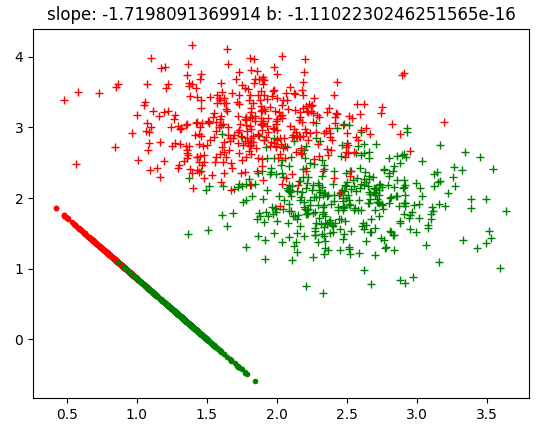
\includegraphics[scale=0.5]{training}
					\centering
				\caption{The class data is plotted along the line that maximizes the separation 
				between the classes.}
			\end{figure}

\section{Questions}
	\subsection{Show that maximization of the class separation criterion given by 
		$L(\lambda, w) = w^{T}(m_{2} - m_{1})  + \lambda(w^{T}w - 1)$ with respect to w, using a
		Lagrange multiplier to enforce the constraint $w^{T}w = 1$, leads to the result that 
		$w \propto (m_{2} - m_{1})$.}
		
		From the definition of the between-class covariance matrix, we know $S_{B}$ is always 
		a scalar of $m_{2} - m_{1}$. When we derive w.r.t. w, we get:
		\[\frac{\partial w}{\partial L} = (m_{2} - m_{1}) - \lambda w\]
		
		In order to maximize this value, we can set the partial derivative of $L$ equal to 0,
		and achieve the following result
		\[ (m_{2} - m_{1}) - \lambda w = 0\]
		\[ (m_{2} - m_{1}) = \lambda w \]
		And thus this implies that $w \propto (m_{2} - m_{1})$. 
		%second question
	\subsection{Using eq \ref{eq:eq1} and eq \ref{eq:eq2}, derive the result eq \ref{eq:eq3} for the posterior class
		probability in the two-class generative model with Gaussian densities, and verify the
		results eq \ref{eq:eq4} and eq \ref{eq:eq5} for the parameters w and $w_{0}$.}
		\begin{equation}
			\label{eq:eq1}
			\frac{1}{1 + exp(-\alpha) = \sigma(\alpha)}
		\end{equation}
		\begin{equation}
			\label{eq:eq2}
			a = ln\frac{p(x|C_{1})p(C_{1})}{p(x|C_{2})p(C_{2})}	
		\end{equation}
		\begin{equation}
			\label{eq:eq3}
			p(C_{1}|x) = \sigma(w^{T}x + w_{0})
		\end{equation}
		\begin{equation}
			\label{eq:eq4}
			w = \sum_{}^{-1}(\mu_{1} - \mu_{2})
		\end{equation}
		\begin{equation}
			\label{eq:eq5}
				w_{0} = -\frac{1}{2}\mu^{T}_{1}\sum_{}^{}^{-1}\mu_{1} + \frac{1}{2}\mu_{2}^{T}\sum_{}^{}^{-1}\mu_{2} + ln\frac{p(C_{1})}{p(C_{2})}
		\end{equation}

		The posterior class probability is directly related to the \textbf{sigmoid function} becasue since 
		all the real numbers live in (0,1), then a value closer to 1 will mean a higher chance p is in $C_{1}$. 
		Thus, our input $w^{T}x + w_{0}$ will directly determine how confident we are in x belonging in $C{1}$,
		which shows that these two are equal.

		For eq 4 and eq 5, assuming an equal covariance matrix for both classes, the square values will
		cancel out once the vector multiplications are done, and thus eq. 4 verifies $ w_{0}$. 
		\end{document}
